

%%%%%%%%%%%%%%%%%%%%%%%%%%%%%%%%%%%%%%%%%%%%%%%%%%%%%%
\section{Design / Proposed Approach}
\label{sec:design}

\subsection{Overview and Goals}
In our initial system, "Iroko", a centralized controller regulates all 
node traffic by rate-limiting end-hosts. We have opted for a centralized 
manager in favor of a distributed protocol to leverage the advantages of a 
global network view.~\footnote{For now, we do not expect our design to scale up 
to thousands of switches. Iroko is intended for small to mid-tier size data 
centers, which may benefit from a simplistic, centralized scheduling model.}
By polling each switch individually for port and utilization statistics we are 
able to infer a global traffic matrix, which we can amalgamate with static 
routing and topology information. 

Iroko attempts to provide minimal congestion and low average access latency. Reducing 
network-global packet loss and jitter is the priority and objective function of 
the arbiter, which will enforce these goals by restricting host bandwidth. In 
an ideal Iroko system, packet-loss will only rarely, if ever, occur. In respect 
to the no free lunch theorem we aim to trade off maximum bandwidth utilization for 
optimal system stability and reliable latency.

It is important to note that routing decisions are not in the current scope of 
Iroko. While it may certainly be beneficial to include dynamic and adaptive 
routing decisions in a predictive scheduler, we do not include these features 
in the current system due to time and complexity limitations. Iroko operates on 
static flow routes defined and generated by ECMP. It is assumed that these 
routes will not vary substantially and that the computed ECMP forwarding hash 
is consistent.

\subsection{Adapting traffic flow}

The controller will dynamically adjust bandwidth allocations to ensure that hosts 
requiring more bandwidth are allocated it, while host that are not currently 
utilizing all their allocated bandwidth have their allocated bandwidth reduced. 
To avoid starving hosts, some small amount of bandwidth must always be 
allocated to a given host even if it not utilizing network resources. Thus, the 
network, by design, will never reach 100\% utilization.

Conversely however one should rarely see dropped packets due to network 
congestion. Furthermore, the controller must be able to react quickly to 
changing bandwidth needs for hosts. Ideally, using a predictive method.


\subsection{Reinforcement Learning}
In order to make predictive rate-limiting decisions per host, we treat rate-limiting as a reinforcement learning problem. In reinforcement learning, an agent (in our case the arbiter) performs actions 
in the environment and receives a reward signal from the environment to adjust 
its decisions in the next epoch ~\cite{Sutton:1998:IRL:551283}. The reward is 
generally used to represent the goal an agent is trying to achieve. The agent 
can freely choose whatever actions are necessary to achieve this goal 
~\cite{Sutton:1998:IRL:551283}.

The environment in this case is defined as the statistics collected from each 
switch and the current end-host to rate limit. This decision is based on the fact that these data are easy to collect and provides a current snapshot of the performance of the data center. Using this representation, we take full advantage of all the information provided in our data center.

We wish to optimize over the packet loss, and define the reward to be good (+1) if there is no loss and bad (-1) if there is any loss.  One limitation of the current reward signal is it's inability to distinguish cases when loss is 0 because no bandwidth was used in the epoch. This means, a more intricate reward functions can be devised for  a future work.

Given the data center assumption, the number of end-hosts is known in the 
topology. We define our arbiter's actions as a single continuous value which will either increase 
decrease, or maintain the allocated bandwidth to different end hosts. A continuous value allows our agent to make direct rate-limiting decisions, and reinforcement learning algorithms have been devised to learn continuous value actions such as this ~\cite{DDPG}. 

Thus we frame our problem as one which can now be solved using techniques in reinforcement learning. Given full representation of our environment and 
actions, we will store the state-action value, also referred to as the Q(s,a) function,  in an artificial neural network. The Q(s,a) function 
stores the reward signal information that is used to make future action choices. We chose an artificial neural network to approximate this function, because of they are theoretically proven function approximators ~\cite{Cybenko1989} which have made intractable environmental representations manageable~\cite{Sutton:1998:IRL:551283}.



\subsection{Controlling traffic flow}
Our future research goal for Iroko is to rate-limit on the granularity of the IP protocol, allowing us 
to restrict traffic to specific hot regions and to package flows into groups.
End-hosts will be guaranteed a limited amount of bandwidth which they may send to 
each destination address. The traffic window size for any flow will be calculated 
based on the host's current traffic availability. Total bandwidth of a group of 
flows may never exceed the imposed bandwidth limitation, but nodes are free to 
distribute the allocated resources on singular subflows.

Iroko would enforce these bandwidth and access limitations by assigning "tokens" to nodes. These tokens are plain information packets 
specifying the affected destination address flow, its bandwidth guarantee, and 
the expiration time. Tokens act as the rate-limiter of the system and form a 
queue each end-host will cycle through.

When a node opens a flow, it will look up the current bandwidth restriction for 
the destination IP in its token database and calculate the maximum congestion 
window possible for the particular TCP connection. In our simple design, flows 
are always assigned a fair fraction.

Once a token has expired for a particular flow-group, the restrictions of the 
next token in the queue will be applied. This mechanism is the underlying basis 
for a predictive access control algorithm and does not require any application 
level modification. On end-hosts, only the transport layer services will have 
to be modified.

\begin{figure}
\centering
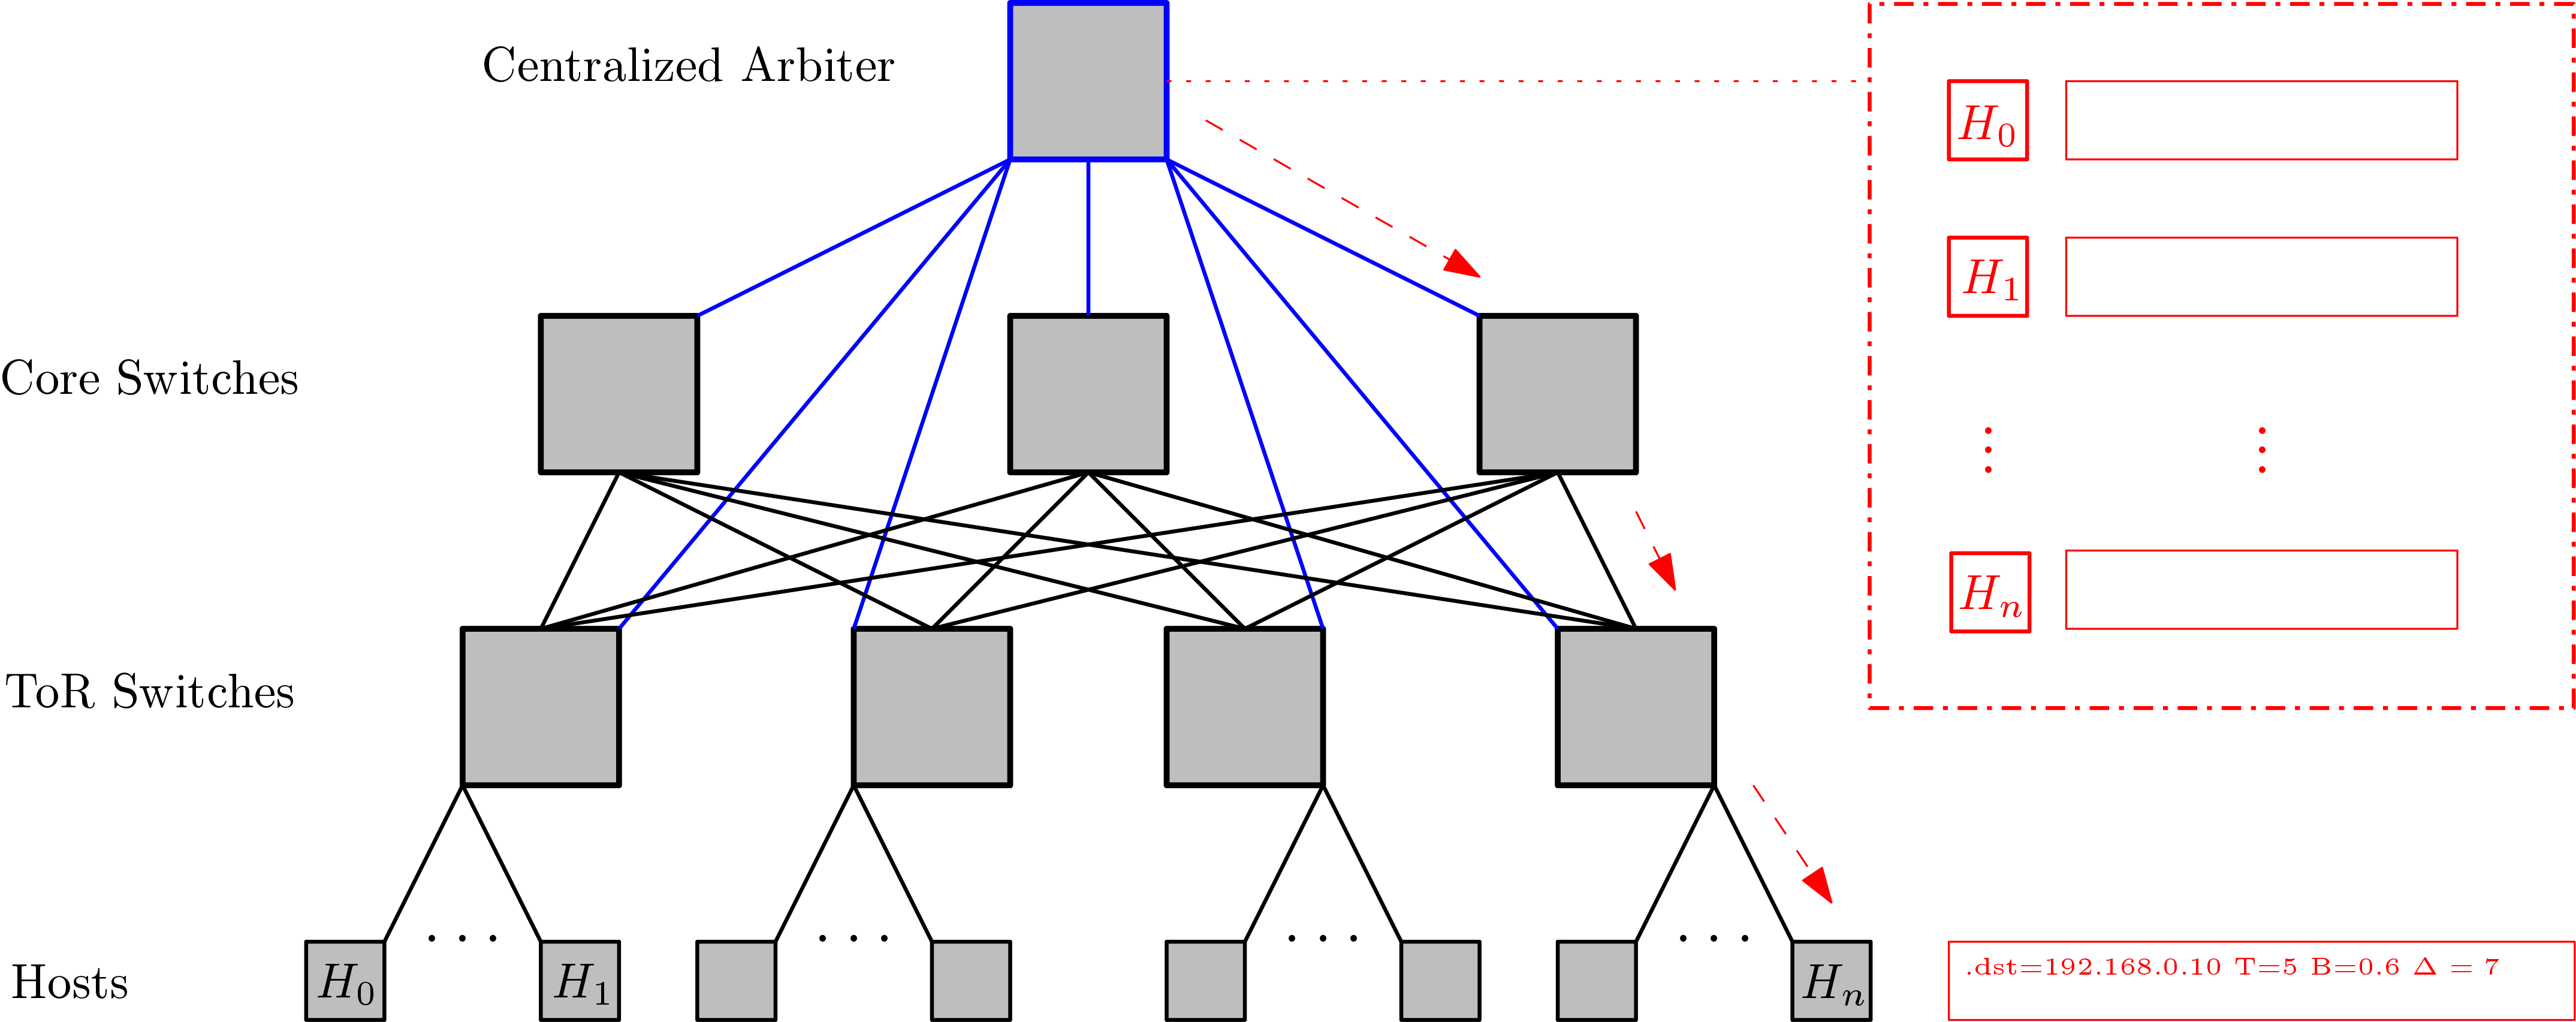
\includegraphics[width=1\linewidth]{Topology3}
\caption{Simple sketch of the Iroko architecture. A central scheduler maintains 
a consistent view of the current network activity and computes the optimal 
end-host bandwidth distribution. Bandwidth is enforced at end-hosts on a per-IP 
basis.}
\label{fig:Topology3}
\end{figure}


%Using this model, we hope to achieve near 0% packet loss and provide a 
%%solution that gets somebody fired at google for not having tried it first.

